
\section{Image classification}


\begin{frame}
	\frametitle{What do you see?}

	\centering
      	\begin{figure}
               	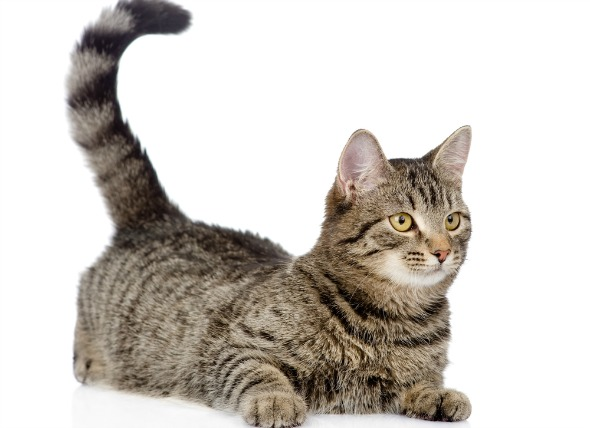
\includegraphics[width=0.75\textwidth]{Pics/cat_generic.jpg}
        \end{figure}

\end{frame}

\begin{frame}
        \frametitle{What does the computer see?}

        \centering
        \begin{figure}
                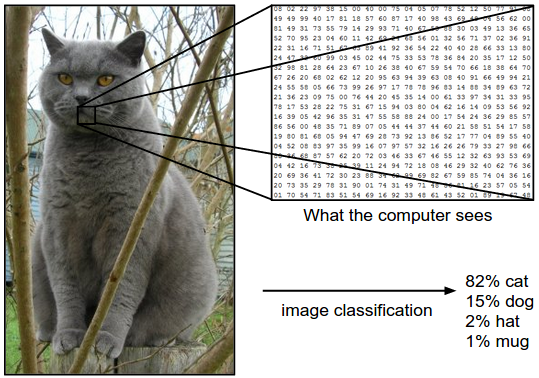
\includegraphics[width=0.7\textwidth]{Pics/cat_computer.png}
        \end{figure}

	Is it THAT difficult?

\end{frame}

\begin{frame}
	\frametitle{Challenges}

	\centering
        \begin{figure}
                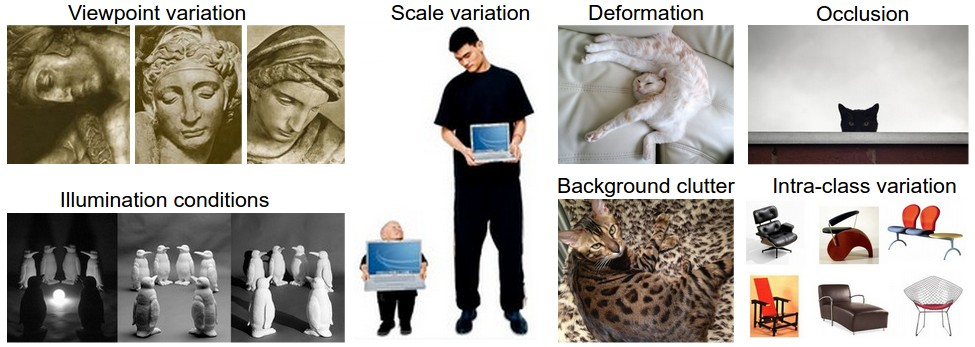
\includegraphics[width=0.9\textwidth]{Pics/challenges.jpeg}
        \end{figure}

	\begin{itemize}
		\item invariant to the cross product of all these variations
		\item retaining sensitivity to the inter-class variations
	\end{itemize}

\end{frame}

\begin{frame}
	\frametitle{Data-driven approach}

	\centering
        \begin{figure}
                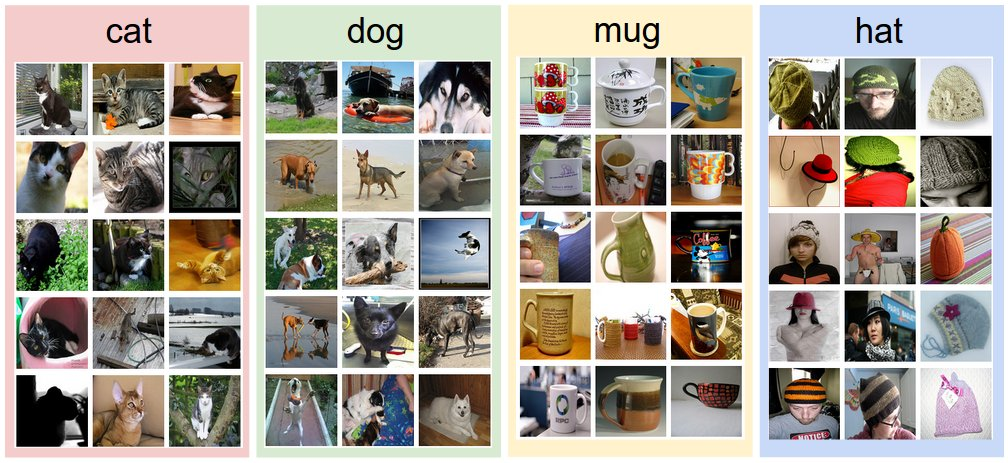
\includegraphics[width=0.7\textwidth]{Pics/trainset.jpg} \\
        \end{figure}

	We need a (large) training dataset of labeled images. 

\end{frame}

\begin{frame}
	\frametitle{Pipeline for image classification}

	\centering
        \begin{figure}
                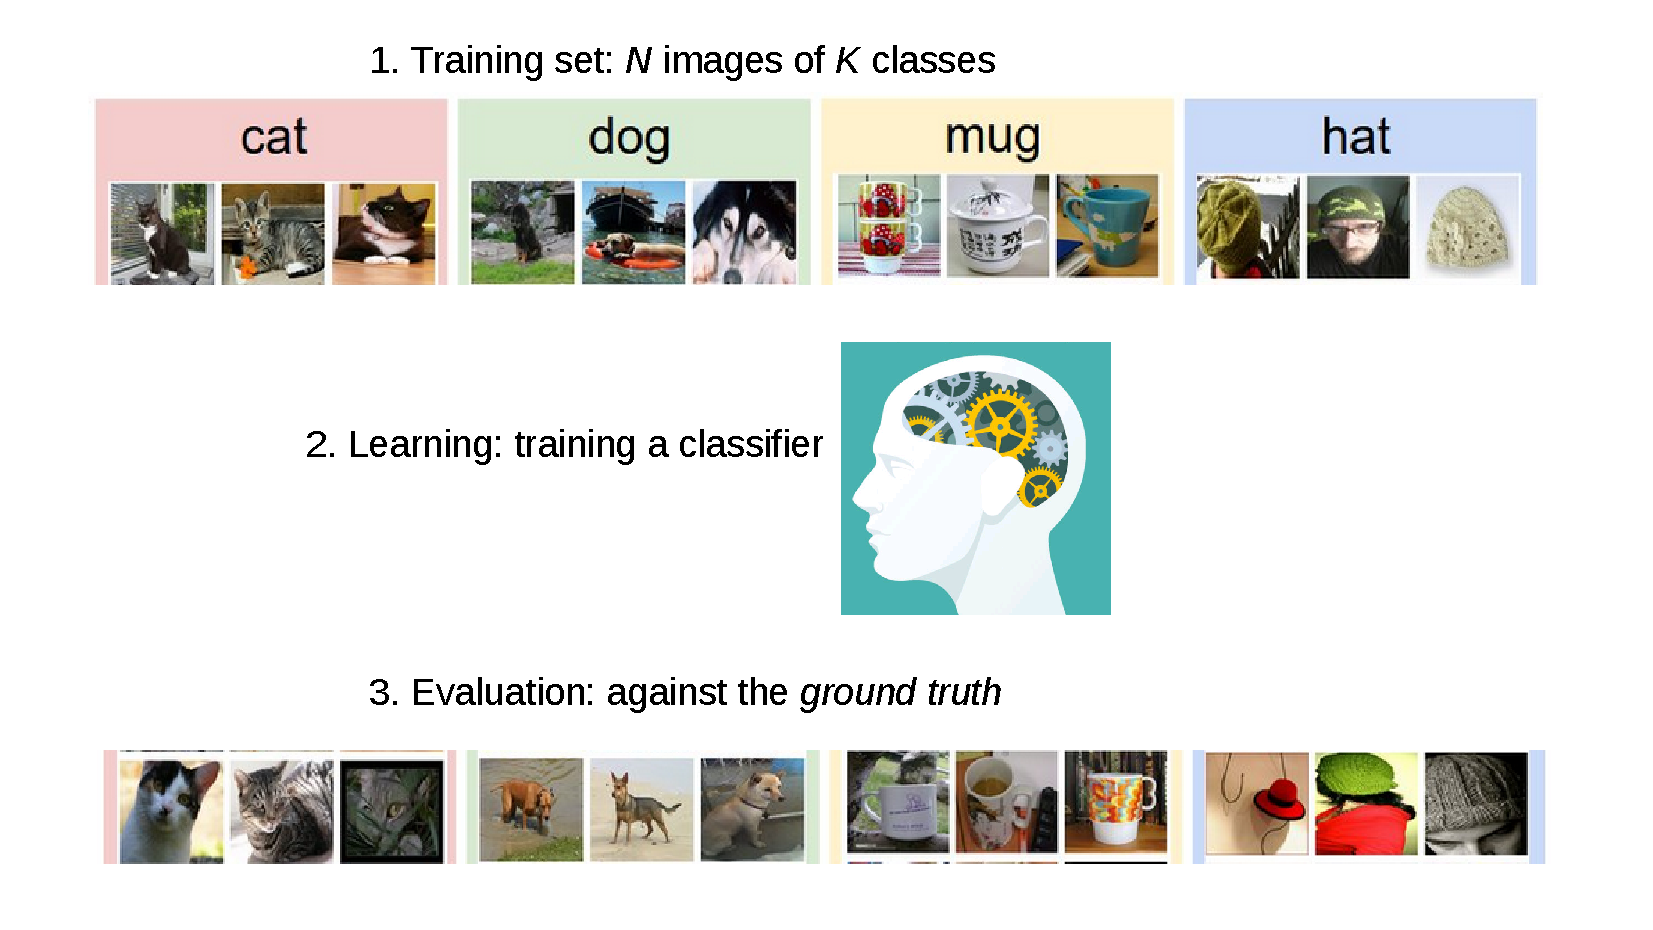
\includegraphics[width=0.9\textwidth]{Pics/pipeline.pdf}
        \end{figure}

\end{frame}

\begin{frame}
	\frametitle{Nearest Neighbour Classifier}

	\centering
        \begin{figure}
                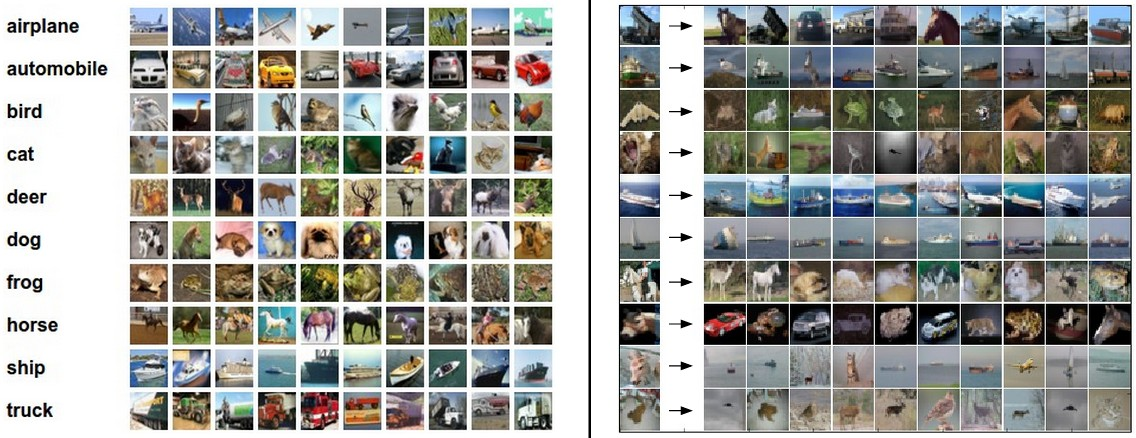
\includegraphics[width=0.9\textwidth]{Pics/nn.jpg} \\
                \caption{CIFAR-10 dataset: 60k tiny images of 10 classes.}
        \end{figure}

	The nearest neighbour classifier will take a test image, \textbf{compare} it to every single one 
	of the training images, and predict the label of the closest training image.

\end{frame}

\begin{frame}
        \frametitle{Nearest Neighbour Classifier}

        \centering
        \begin{figure}
                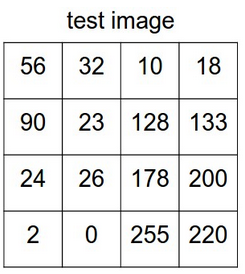
\includegraphics[width=0.4\textwidth]{Pics/nn1.png}
        \end{figure}

\end{frame}

\begin{frame}
        \frametitle{Nearest Neighbour Classifier}

        \centering
        \begin{figure}
                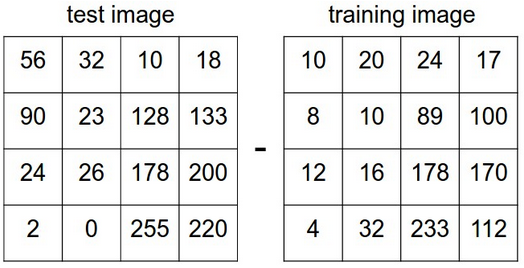
\includegraphics[width=0.7\textwidth]{Pics/nn2.png}
        \end{figure}

\end{frame}

\begin{frame}
        \frametitle{Nearest Neighbour Classifier}

        \centering
        \begin{figure}
                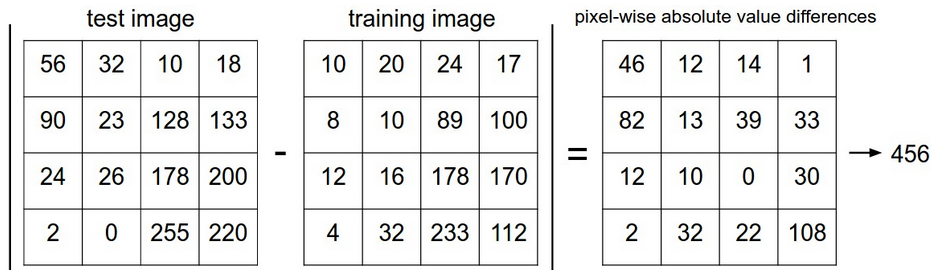
\includegraphics[width=0.8\textwidth]{Pics/nn3.png}
        \end{figure}

\end{frame}

\begin{frame}
	\frametitle{The choice of distance}

	L1 distance: $d_1(I_1,I_2)= \sum_{pixel} |I_1^p - I_2^p|$
	\vskip 0.5cm
	L2 distance: $d_1(I_1,I_2)= \sqrt{ \sum_{pixel} (I_1^p - I_2^p)^2 } $

	\vskip 1cm

	What's their accuracy?\\
	What's human accuracy?\\
	What's state-of-the-art neural networks' accuracy?

\end{frame}

\begin{frame}
	\frametitle{k-Nearest Neighbour Classifier}

	\centering
        \begin{figure}
                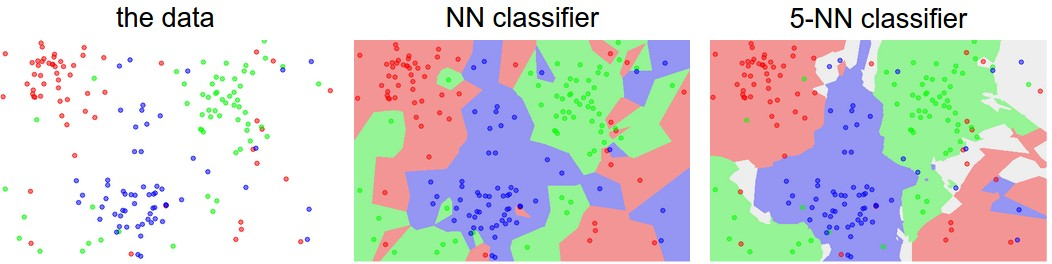
\includegraphics[width=0.9\textwidth]{Pics/knn.jpeg} \\
                \tiny{\caption{An example of the difference between Nearest Neighbor and a 5-Nearest Neighbor classifier, using 2-dimensional points and 3 classes (red, blue, green).}}
        \end{figure}

	What value of \textit{k} should we use? Which distance?

\end{frame}

\begin{frame}
	\frametitle{Hyperparameter tuning}

	\begin{columns}
		\column{0.5\textwidth}
		\begin{figure}
                	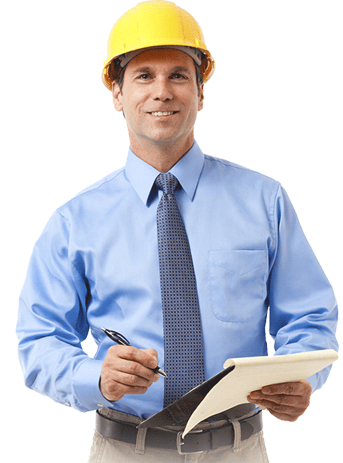
\includegraphics[width=0.6\textwidth]{Pics/engineer.png} \\
        	\end{figure}
		\column{0.5\textwidth}
		The engineer says: "We should try out many different values and see what works best."
	\end{columns}
	\vskip 0.3cm
	\centering
	Agree or disagree?

\end{frame}

\begin{frame}
        \frametitle{Validation test}

        \begin{columns}
                \column{0.5\textwidth}
                \begin{figure}
                        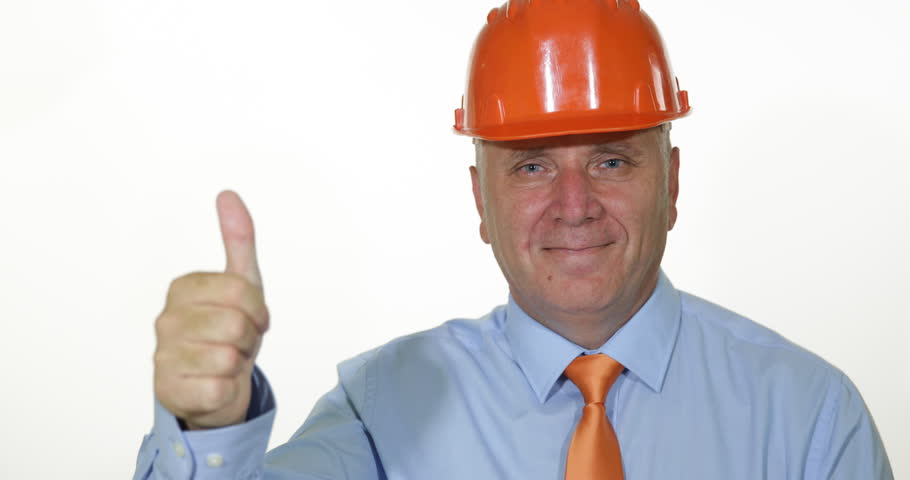
\includegraphics[width=0.9\textwidth]{Pics/good_engineer.jpg} \\
                \end{figure}
                \column{0.5\textwidth}
                The good engineer says: "Evaluate on the test set only a single time, at the very end."
        \end{columns}

	\begin{itemize}
		\item Split your training set into training set and a validation set. 
		\item Use validation set to tune all hyperparameters. 
		\item At the end run a single time on the test set and report performance.        
	\end{itemize}

\end{frame}

\begin{frame}
	\frametitle{Data splits}

	\begin{figure}
		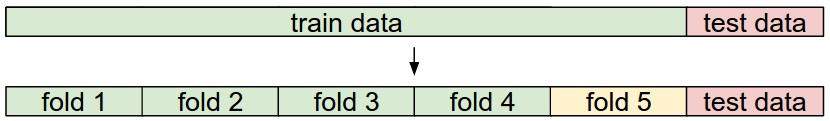
\includegraphics[width=0.9\textwidth]{Pics/crossval.jpeg} \\
		\caption{The training set is split into folds: 1-4 become the training set while 5 is the validation set used to tune the hyperparameters.}
     	\end{figure}

	Where is the Nearest Neighbour classifier spending most of its (computational) time?

\end{frame}

\begin{frame}
	\frametitle{Wrap up}
	
	\begin{itemize}
		\item the problem of image classification: predicting labels for novel test entries
		\item training set vs testing set
		\item a simple Nearest Neighbor classifier requires hyperparameters
		\item validation set to tune hyperparameters
		\item Nearest Neighbor classifier has low accuracy (distances based on raw pixel values!) and is expensive at testing
	\end{itemize}

	Our aim: a solution which gives 90\% accuracy, discards the training set once learning is complete, and evaluates a test image in less than a millisecond!

\end{frame}





